\chapter[Introdução]{Introdução}

A Engenharia de Requisitos é um ramo da Engenharia de \textit{Software} que se preocupa com os objetivos do mundo real, funções e restrições dos sistemas de \textit{software}, fazendo parte do ciclo de desenvolvimento do \textit{software} e sendo crucial para o sucesso geral e precisão do sistema desenvolvido. Também se preocupa com a relação desses fatores com caracterizações exatas do comportamento do \textit{software} e com a sua evolução ao longo do tempo \cite{elliott2012software}.

Esta desempenha um papel significativo no desenvolvimento de aplicativos de \textit{software} pelo fato de fornecer uma maneira de entender e descrever os problemas que requerem uma solução de \textit{software}. Isso é crucial para deter as necessidades dos usuários e especificar tais necessidades como requisitos de \textit{software} \cite{elliott2012software}. É uma área de suma importância, pois é necessária para melhorar as taxas de sucesso de um projeto.

A elicitação, a análise, a modelagem e a validação são processos essenciais dentro da Engenharia de Requisitos que ajudam a cumprir o propósito de um \textit{software}. Além disso, a Engenharia de Requisitos documenta o sistema, identifica todas as partes interessadas e suas preocupações e apresenta essas informações de uma forma que possam ser analisadas e, eventualmente, implementadas \cite{elliott2012software}.

Por se tratar de uma área que se encontra entre o abstrato e o concreto, Westfall \cite{westfall_5w2h} em seu estudo busca definir os diferentes porquês da existência da Engenharia de Requisitos:

\begin{itemize}
    \item O que é: são os requerimentos responsáveis pela definição do que o \textit{software} deve fazer (\texit{requisito funcional}\footnote{Declarações de serviços que o sistema deve prover, como deve reagir para entradas e como deve se comportar em situações especificas \cite{sommerville2011}.}) e possuir (\textit{requisitos não funcionais}\footnote{Restrições aos serviços ou funções oferecidas pelo sistema. Aplicam-se ao sistema como um todo \cite{sommerville2011}.}) para agregar valor para os seus \textit{stakeholders}\footnote{Grupo de pessoas interessadas no produto, podendo ser cliente, usuários etc.}; Existem vários níveis e tipos diferentes de requisitos, que são mostrados na figura \ref{lev_tipo_req}:
    
    \begin{figure}[htb]
        \begin{center}
            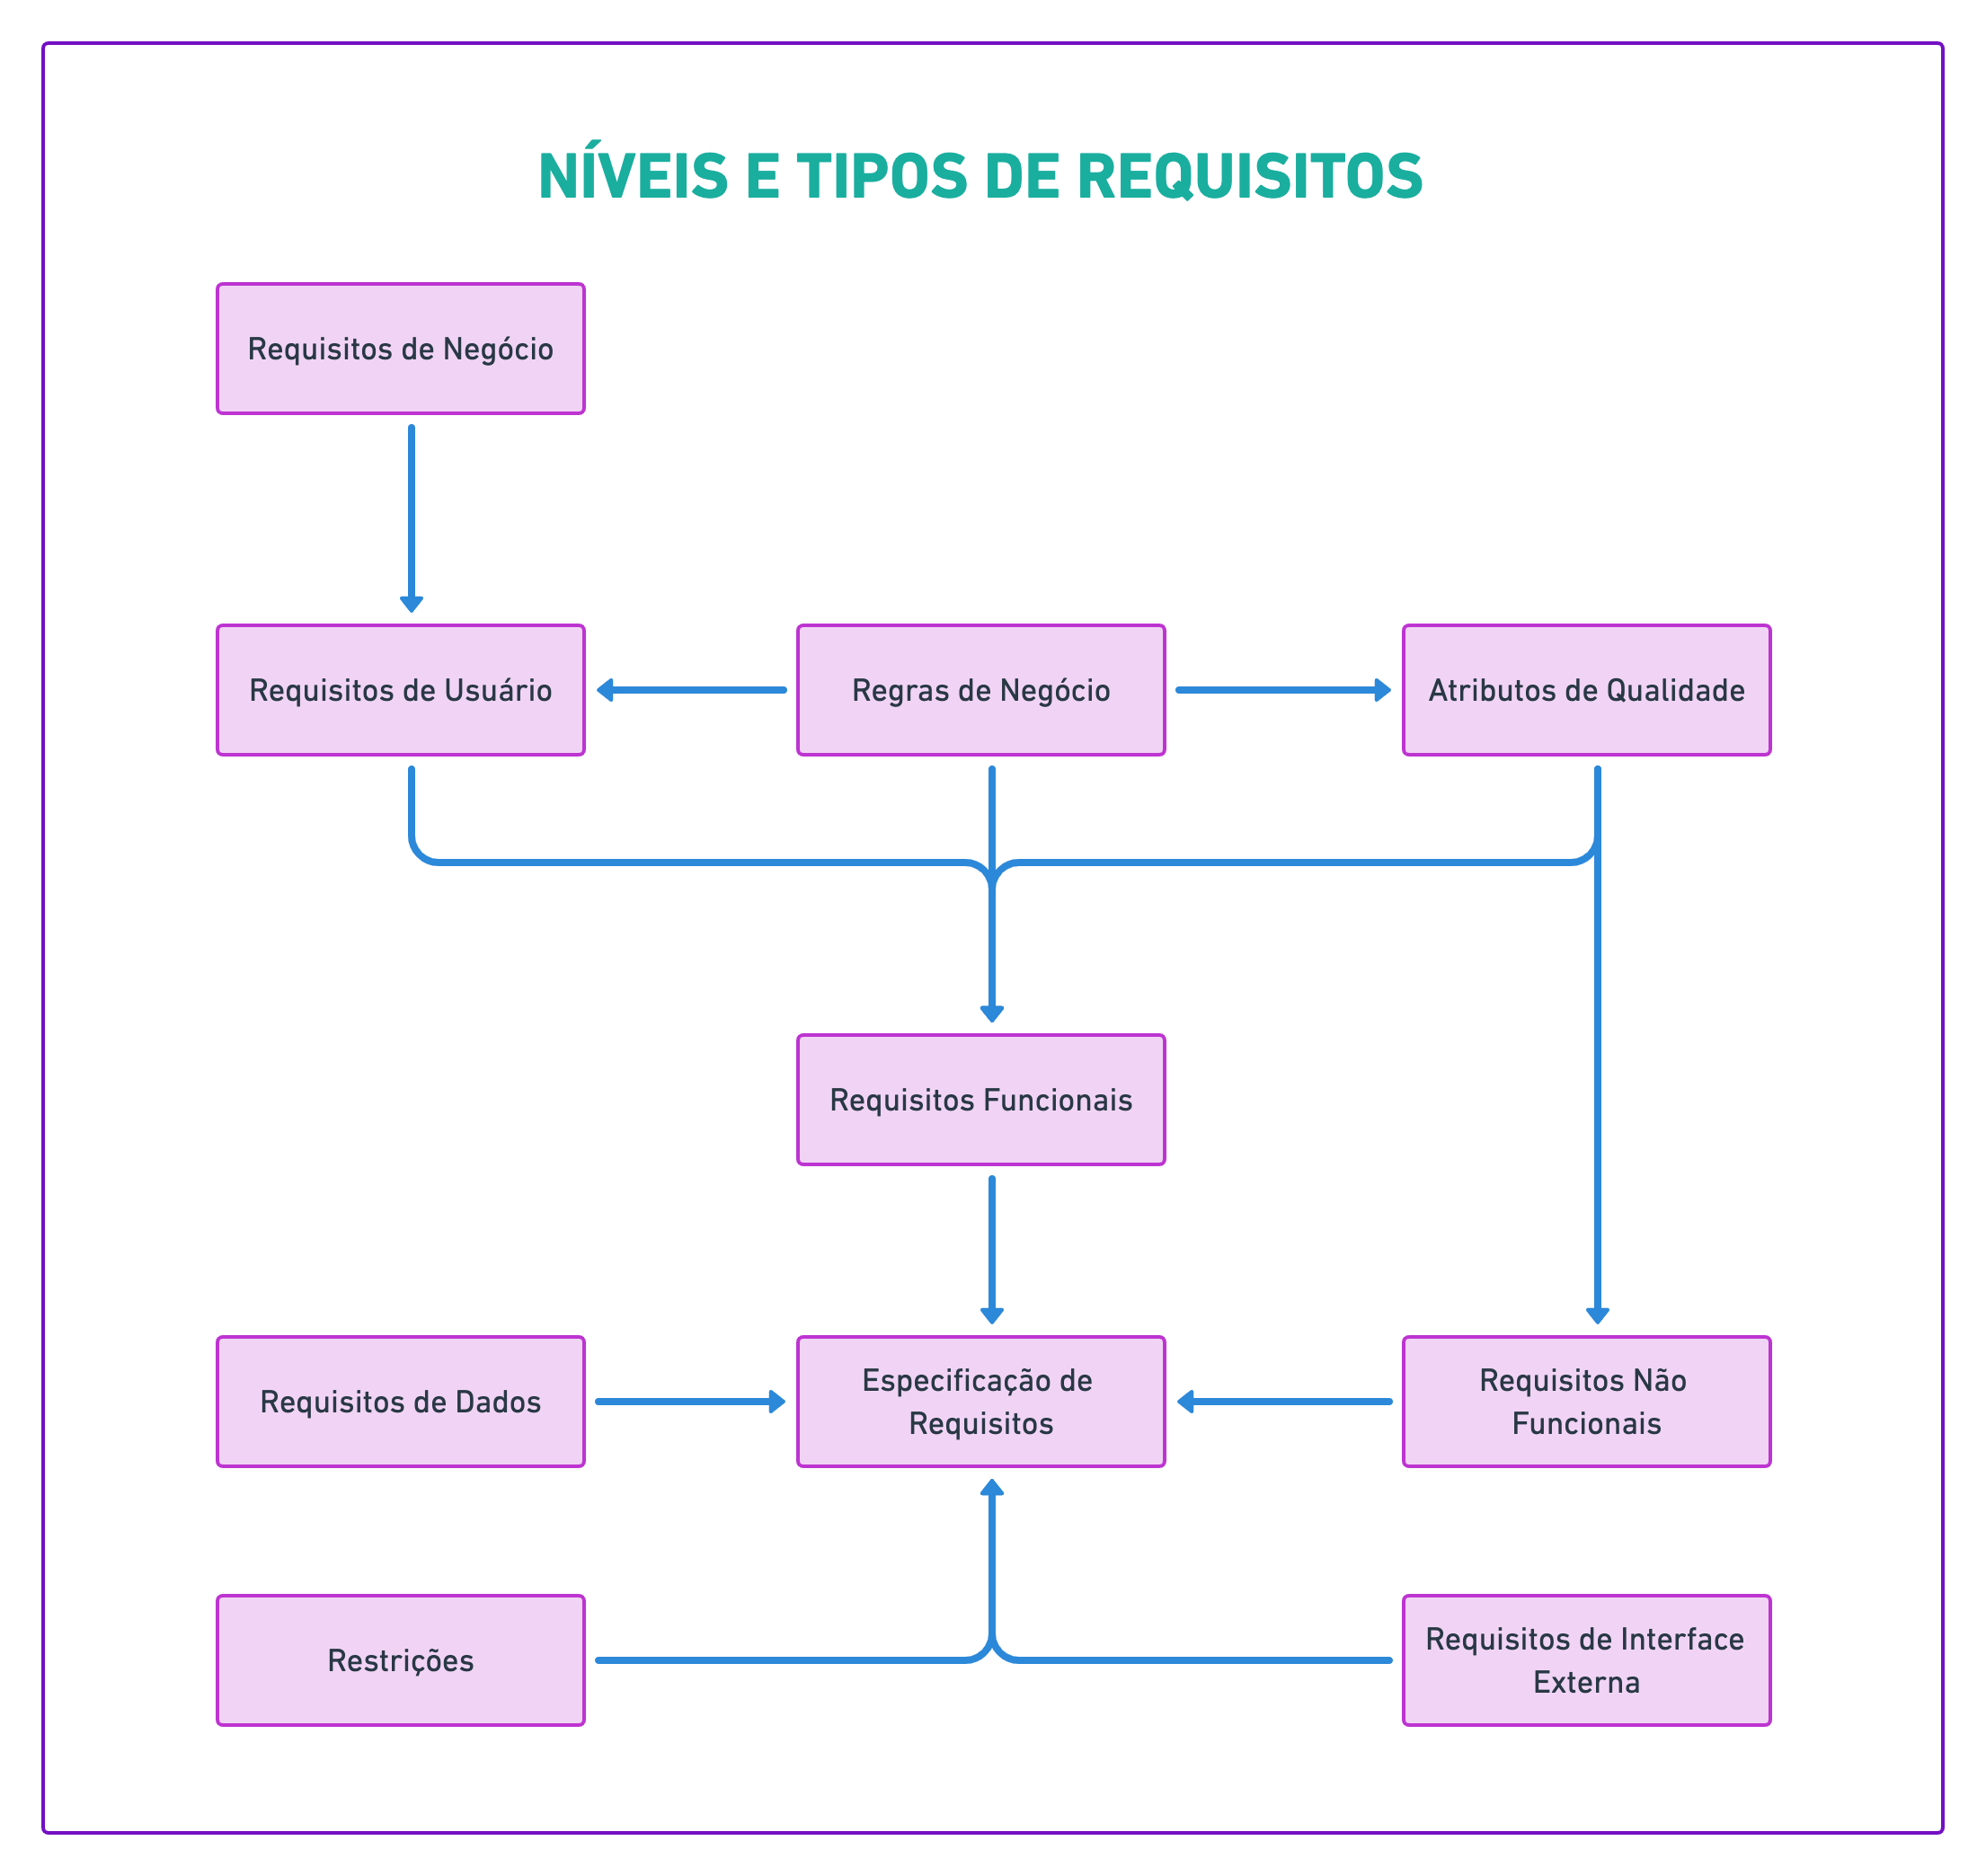
\includegraphics[width=10cm, height=8cm, keepaspectratio]{figuras/lev_tipo_req.png}
            \caption{{Níveis e Tipos de Requisitos. \cite{westfall_5w2h}}}
            \label{lev_tipo_req}
        \end{center}
    \end{figure}
    
    \begin{itemize}
    
    \item Os requisitos de negócio definem, de forma direta, quais são os problema que devem ser resolvidos e definir por que o produto de \textit{software} está sendo desenvolvido;
    
    \item Os requisitos de usuário têm o objetivo de visualizar as funcionalidades do produto de \textit{software} a partir da perspectiva do usuário. De forma resumida, eles definem o que o \textit{software} deve realizar para que os usuários atinjam seus objetivos.
    
    \item Os requisitos funcionais de produto definem as funcionalidades do software que devem ser implementadas para que os usuários consigam realizar suas tarefas de forma fácil.
    
    \item As regras de negócio são declarações sobre a forma da empresa fazer negócio, ou seja, elas refletem as políticas, os padrões, as práticas, os regulamentos e as diretrizes de negócio.
    
    \item Os atributos de qualidade no nível de usuário definem requisitos não funcionais que determinam o produto de \textit{software}. Incluem confiabilidade, disponibilidade, segurança, manutenibilidade, portabilidade, usabilidade etc.
    
    \item Os requisitos de interface externa, de forma objetiva, definem o fluxo de informações através de interfaces compartilhadas.
    
    \item As restrições têm o objetivo de mostrar quais destas foram colocadas pelo fornecedor ao projetar e desenvolver o \textit{software}.
    
    \item Os requisitos de dados definem os itens de dados específicos que devem ser introduzidos como parte do produto de \textit{software}.
    
    \end{itemize}
    
    \item Por que serve: de acordo com Brooks \cite[p.~199]{brooks1995mythical} "A parte mais difícil da construção de um sistema de \textit{software} é decidir precisamente o que deve ser feito. Nenhuma outra parte do trabalho conceitual é tão  custoso quanto estabelecer detalhadamente os requisitos técnicos, incluindo todas as interfaces para os usuários, para os computadores, e para os outros sistemas do \textit{software}. Nenhuma outra parte do trabalho prejudica tanto o sistema se for feita de maneira errada. Nenhuma outra parte é tão difícil de ser retificada posteriormente." Assim, pode-se entender o quão crítico é esse contexto o qual está inserido esse trabalho;
    
    \item Para quem: os stakeholders são indivíduos que afetam ou que são afetados pelo produto de \textit{software} e, portanto, possuem um nível de influência sobre o produto. Dentro desse contexto, existem diferentes perspectivas relacionada à atuação de cada indivíduo:
    
    \begin{itemize}
        \item Os Analistas de Requisitos são essenciais dentro dessa área pelo fato deles serem responsáveis pela elicitação, análise e especificação dos requisitos, além de comunicar os requisitos aos desenvolvedores e as partes interessadas;
    
        \item Os Arquitetos de \textit{Software} são essenciais por criarem toda a arquitetura do \textit{software} a partir dos requisitos elicitados e por dizerem como o \textit{software} vai ser implementado;
    
        \item Já os desenvolvedores são responsáveis por implementarem o produto de \textit{software}. São eles os responsáveis em traduzir os requisitos em funcionalidades concretas;
    
        \item Os Testadores de \textit{Software} têm o objetivo de usar os requisitos elicitados como base e criar casos de teste para que o produto de \textit{software} seja testado sob condições específicas, afim de detectar defeitos para que, após testarem, passem confiabilidade de que o produto de \textit{software} esteja funcionando de acordo com as características estabelecidas;
    
        \item Os Gerentes de Projeto são responsáveis pelo planejamento e monitoramento de todos os envolvidos no projeto, além de guiar o time de desenvolvimento de \textit{software} para que o produto final seja entregue com todos os requisitos definidos anteriormente;
    
        \item O Gerente do Produto é uma peça fundamental dentro desse processo, pois revisa todas as mudanças propostas, analisa os riscos e os impactos que podem vir a ocorrer e aprovam e desaprovam quaisquer mudanças, garantindo que essas mudanças foram implementadas e validadas.
    \end{itemize}
    
    \item Quando: a maior parte do processo da engenharia de requisitos é feita nas primeiras fases do ciclo de vida do produto, contudo não deve ser restrito somente a esse período, uma vez que novos requisito vão surgindo e o projeto deve se adaptar as novas realidades, pois deve ser um processo iterativo. Esse aspecto está ligado ao gerenciamento de requisitos que deve avaliar novas requisições, avaliar os riscos e impactos que acarretará, aceitar ou não e, finalmente, implementar essa nova funcionalidade. Durante a fase de desenvolvimento, estes requisitos devem ser usados como critérios para testar o produto e validar a correta implementação das funcionalidades. Os requisitos de negócio devem ser os primeiros a serem modelados, seguidos dos requerimentos de usuário e, por fim, os de produto;
    
    \item Como: A engenharia de requisitos de \textit{software} é um processo bem definido, com etapas claras e recheadas de documentações que possam registrar e orientar o desenvolvimento do produto. O desenvolvimento e a gerência dos requisitos são dois grandes processos dentro deste escopo. A figura \ref{eng_req_flux} representa bem essas etapas e subetapas do processo da engenharia de requisitos que vão ser melhor especificadas no decorrer deste trabalho.
    
    \begin{figure}[htb]
        \begin{center}
            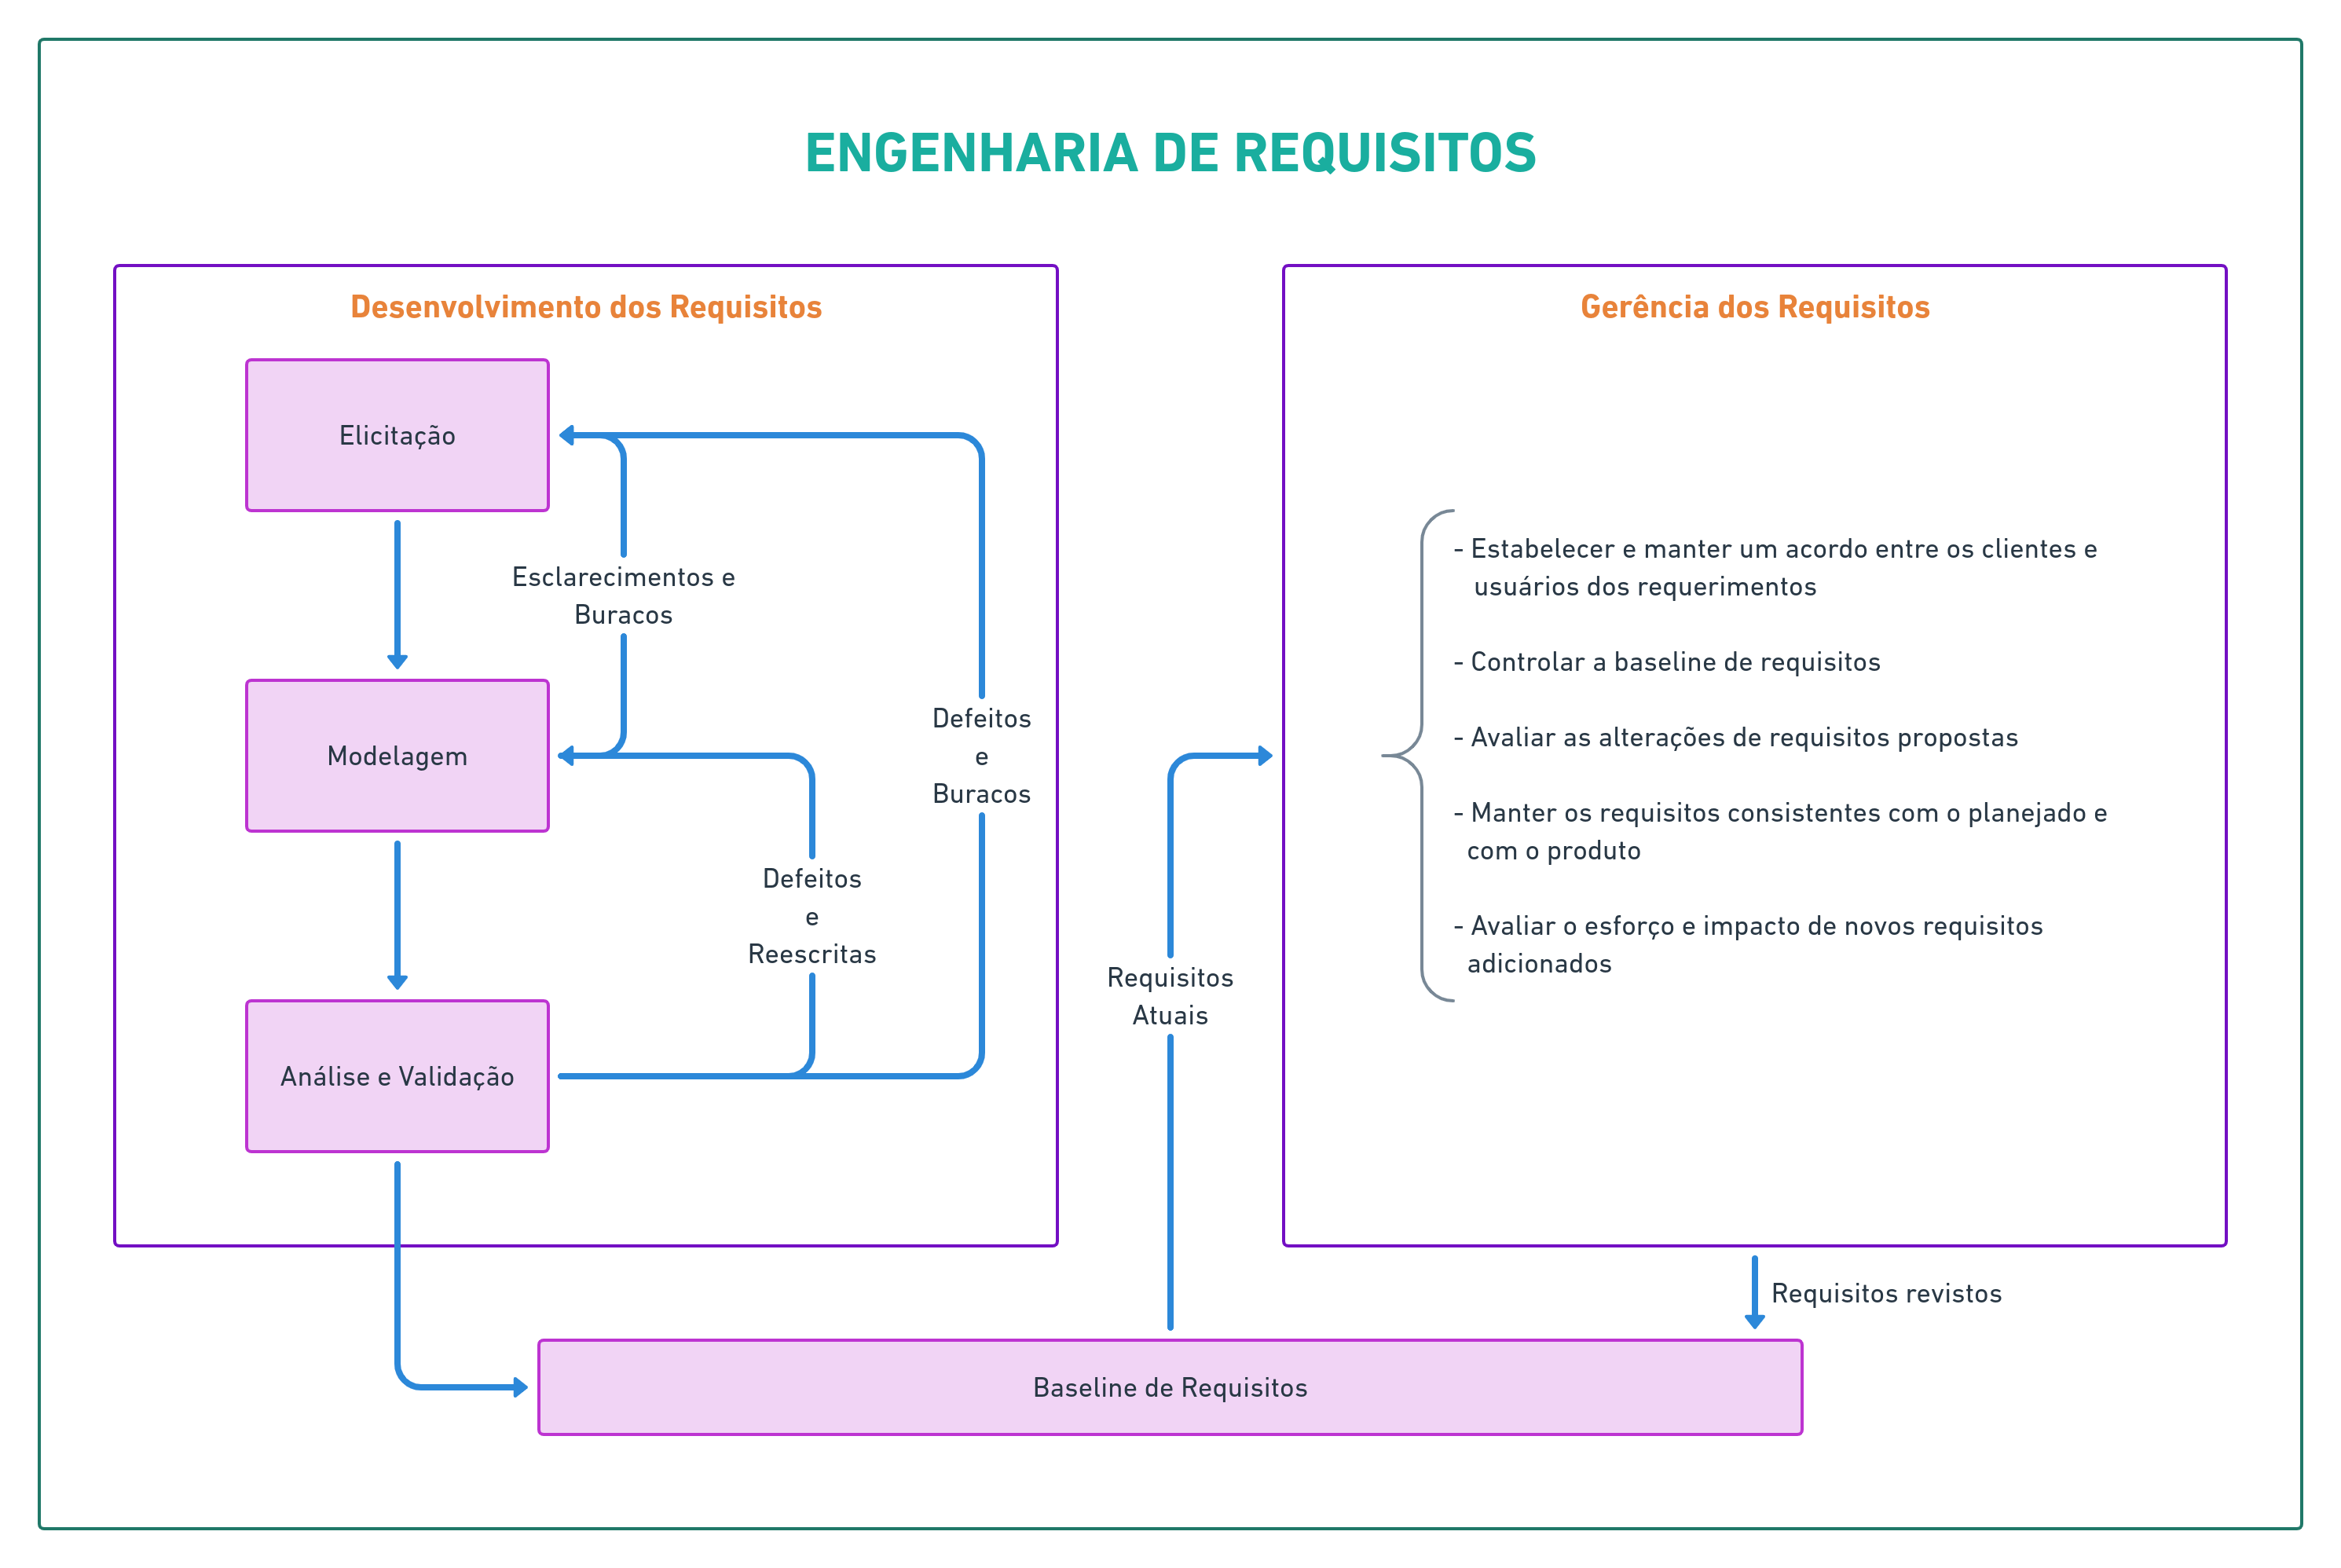
\includegraphics[width=10cm,height=10cm,keepaspectratio]{figuras/Introducao/eng_req_fluxo.png}
            \caption{{Fluxo da Engenharia de Requisitos. Adaptado de \cite{westfall_5w2h}}}
            \label{eng_req_flux}
        \end{center}
    \end{figure}
    
    Por fim, a área de requisitos é essencial dentro do ciclo de desenvolvimento de \textit{software}, porém, por muitas vezes, é negligenciada pelo fato de possuir tantos processos a serem seguidos, o que impacta diretamente nos custos e no resultado final do produto. Para exemplificar, ocorreu um caso em Londres 
    
\end{itemize}
